\section{24.09.2014 - Amplificatori Operazionali Reali - Prima Parte}

In questa esperienza studieremo un amplificatore operazionale $\mu$A$741$ considerandolo reale, quindi ne analizzeremo la tensione di offset e le correnti di polarizzazione (\textit{bias currents}).
Ricordiamo che il circuito di alimentazione e di riduzione dei rumori (Figura \ref{gr:costante}) è il medesimo dell'esperienza precedente: per facilitare la comprensione degli schemi circuitali è dunque nascosto.
%Premettiamo che il circuito di alimentazione è lo stesso utilizzato nella precedente esperienza e dunque non ripeteremo le considerazioni e gli schemi circuitali già proposti.
%Inoltre ricordiamo che la circuiteria di alimentazione sugli schemi è stata nascosta per facilitarne la comprensione.

\subsection*{Strumenti e materiali}

\begin{itemize} [noitemsep]
\item Generatore di tensione continua Agilent E3631A (max $\pm \, \SI{25}{\volt}$ o $\pm \, \SI{6}{\volt}$);
\item Multimetro Agilent 34410A a sei cifre e mezza;
\item Un amplificatore operazionale $\mu$A741;
\item Resistenze e capacità di vari valori;
\item un trimmer a un giro da \SI{5}{\kilo\ohm} e uno da \SI{10}{\kilo\ohm}, utilizzati per una prima prova;
\item un trimmer multigiro da \SI{10}{\kilo\ohm};
\item Breadboard e cablaggi vari.
\end{itemize}

\subsection{Tensione di offset}
\label{par2:offset}

In un amplificatore ideale accade che, quando gli ingressi sono entrambi collegati a comune, la tensione di uscita è pari a $0$. Questo fatto si spiega solo se consideriamo all'interno dell'op-amp una perfetta simmetria, attuabile solo se i transistor della circuiteria interna sono uguali in ogni caratteristica. Ovviamente, è impossibile creare degli elementi circuitali che siano perfettamente identici, e ciò causa la perdita della simmetria e l'instaurarsi di una tensione di offset. In questa parte dell'esperienza cercheremo di valutarla.

\subsubsection{Configurazione senza retroazione}

Quando colleghiamo entrambi gli ingressi a comune (come in Figura \ref{cir:open_loop}) l'op-amp vede all'ingresso una differenza di potenziale (ovviamente, fra gli ingressi non c'è, in quanto collegati entrambi a comune) la quale viene amplificata dal guadagno a maglia aperta: come $V_{out}$ avremo dunque un valore diverso da zero. Nel nostro caso l'op-amp andava in saturazione negativa (\SI{-14.3}{\volt}): ciò implica che l'op-amp si comporta come se la tensione all'ingresso invertente fosse maggiore di quella all'ingresso non invertente. Inoltre il valore $V_{out}$ è diverso da \SI{-15}{\volt} utilizzati come alimentazione in quanto il valore di tensione massimo $|V_{out}|$ è leggermente inferiore a alla tensione di alimentazione $-V_{CC}$.

\begin{figure}[ht]
        \centering
        \begin{subfigure}[b]{0.35\textwidth}
                 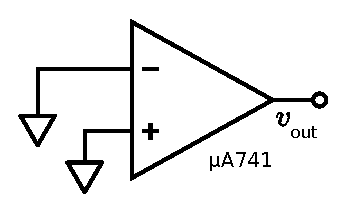
\includegraphics[width=0.70\textwidth]{../E02/latex/open_loop.pdf}
                \caption{Circuito a maglia aperta}
                \label{cir:open_loop}
        \end{subfigure}%
    \quad
        \begin{subfigure}[b]{0.35\textwidth}
               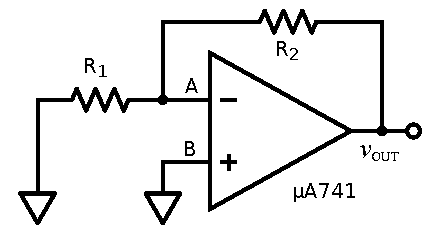
\includegraphics[width=0.70\textwidth]{../E02/latex/inv.pdf}
                \caption{Circuito amplificatore}
                \label{cir:inv}
        \end{subfigure}
     
\end{figure}

Con il circuito in Figura \ref{cir:open_loop} non possiamo quindi ricavare una stima del valore di offset. Per fare ciò dobbiamo ricorrere a un circuito amplificatore come quello in Figura\ref{cir:inv}, che ci permetta di controllare il guadagno.

\subsubsection{Configurazione con retroazione}

Trattiamo per primo il caso \textbf{invertente}. Assumiamo che la tensione nel punto A sia $V_A=V_{off}$ e $V_B=0$. Vale allora che, uguagliando le correnti

$$\frac{V_{off}}{R_1} + \frac{V_{off}-V_{out}}{R_2} = 0$$

da cui si ricava che

$$V_{out}=\left(1+\frac{R_2}{R_1}\right) V_{off}$$

Analogamente si tratta il caso \textbf{non invertente}, assumendo che $V_B=-V_{off}$ e $V_A=0$. L'analisi risulta dunque identica a quella di un amplificatore non invertente, e si ottiene lo stesso risultato del caso invertente. 

Riportiamo nella seguente tabella i valori di offset calcolati, definendo il guadagno come Gain$=1+R_2/R_1$. 

\begin{center}
\begin{savenotes}
\begin{tabular}{c|c|c|c|c|c|c}
$R_1[\si{\ohm}]$ & $R_2[\si{\kilo\ohm}]$ & Gain &$V_{out} [\si{\milli\volt}]$ & $V_{off}$ [\si{\milli\volt}]\\ 
\hline 
$119.8\pm0.1$ & $9.911\pm0.001$ & $83.73\pm0.07$&  $-103.5 \pm 0.5$ & $-1.23 \pm0.01$\\
\hline
$119.8\pm0.1$ & $99.35\pm0.01$ & $830.3\pm0.7$ &$ -1025 \pm 2$ & $-1.2 \pm0.1$\\

\end{tabular}
\end{savenotes}
\end{center}

\begin{wrapfigure}[17]{l}{0.55\textwidth}
  \begin{center}
    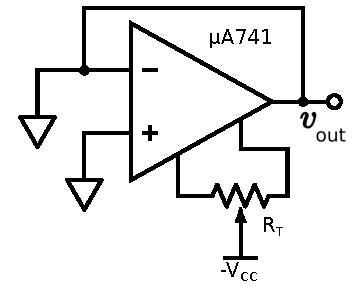
\includegraphics[width=0.280\textwidth]{../E02/latex/trimmer_correction.pdf}
  \end{center}
  \caption{Circuito a guadagno unitario, con trimmer sui piedini 1 e 5 dell'OPAMP per compensare l'offset.}
  \label{cir2:trimmer}
\end{wrapfigure}

Per risolvere il problema dell'offset possiamo servirci di una resistenza variabile ($trimmer$) che posizioneremo tra i piedini 1 e 5 dell'op-amp (appositamente posti dal produttore a questo scopo), e collegandola a $V^-$ come in Figura \ref{cir2:trimmer}. Regolando tale resistenza andremo a generare una contro tensione che bilancerà l'offset. Durante l'esperienza abbiamo provato ad utilizzare trimmer ad un giro da \SI{10}{\kilo\ohm} (oltre che uno da \SI{5}{\kilo\ohm}, che è risultato di valore troppo basso) ma la sensibilità meccanica era troppo bassa per poter azzerare l'offset (la tensione di uscita infatti passava da $\approx$\SI{-14}{\volt} a $\approx$\SI{+14}{\volt}). Abbiamo dunque utilizzato un trimmer multigiro da \SI{10}{\kilo\ohm}, con il quale abbiamo raggiunto la tensione $V_{out}\approx 0$. Abbiamo poi controllato che l'offset fosse effettivamente stato minimizzato riutilizzando il circuito in Figura \ref{cir:open_loop} e ottenendo $V_{out}= (1.3\pm0.2)\si{\volt}$. Ricordando che il guadagno a maglia aperta è di 100-120dB, si nota il buon bilanciamento della tensione di offset.

Come sappiamo la tensione di offset non è però l'unico problema che incontriamo quando usiamo gli op-amp. Infatti ingresso invertente e non invertente sono collegati alle basi di alcuni transistor e, ovviamente, per polarizzarli serve una corrente di base. Gli effetti di tale corrente si sommeranno dunque a quelli dovuti all'offset.

\begin{wrapfigure}[13]{r}{0.55\textwidth}
  \begin{center}
    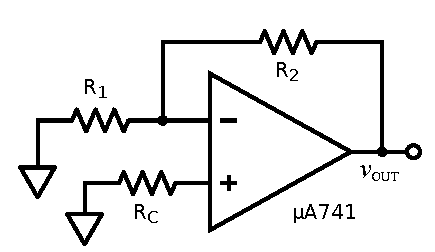
\includegraphics[width=0.280\textwidth]{../E02/latex/current_correction.pdf}
  \end{center}
  \caption{Circuito utilizzato per la stima di $V_{off}$ con la correzione sulle correnti data da $R_C$.}
  \label{cir2:current_correction}
\end{wrapfigure}

Queste correnti di bias, per quanto piccole (\si{\nano\ampere}), giocano un ruolo sull'offset totale. Per minimizzare il loro impatto sul valore della tensione di offset abbiamo inserito fra l'ingresso non invertente e comune una resistenza di compensazione $R_C$ tale da annullare il contributo delle correnti di offset sulla tensione di uscita.

Il valore opportuno di $R_C$ può essere stimato nel modo che segue. Consideriamo la tensione di uscita, che in funzione delle correnti di polarizzazione è

\begin{equation}
V_{out}^{C} = \left( 1+\frac{R_2}{R_1} \right)\left[ \frac{I_{b^-}R_2}{\frac{R_1+R_2}{R_1}} - I_{b^+} R_B\right]
\label{eq2:Vout_currents}
\end{equation}

Si ricava che, supponendo $I_{off} = |I_{b^+}|-|I_{b^-}| \approx 0$ e ponendo $V_{out}^{C}=0$ (annullando così il contributo delle correnti di polarizzazione alla tensione di uscita),

$$R_C=\frac{1}{\frac{1}{R_1} + \frac{1}{R_2}} = R_1 // R_2$$

Riportiamo nella seguente tabella i nuovi valori in questa nuova configurazione (circuito in Figura \ref{cir2:current_correction}):

\begin{center}
\begin{tabular}{c|c|c|c|c|c|c}
$R_C [\si{\ohm}]$& $R_1[\si{\ohm}]$ & $R_2[\si{\kilo\ohm}]$ & Gain & $V_{out}' [\si{\milli\volt}]$ & $V_{off}' [\si{\milli\volt}]$ & $|V_{off}-V_{off}'|[\si{\milli\volt}]$ \\ 
\hline 
$119.4\pm0.1$ & $119.8\pm0.1$ & $9.911\pm0.001$  & $83.73 \pm 0.07$ & $-105.5 \pm 0.5$ & $-1.26 \pm0.01$ & $0.02\pm0.01$ \\
\hline
$119.4\pm0.1$ & $119.8\pm0.1$ & $99.35\pm0.01$  & $830.3\pm0.7$ &$ -1038 \pm 5$ & $-1.2 \pm 0.1$ & $\approx 0$\\
\end{tabular}
\end{center}

Notiamo che le differenze fra i valori della tensione di offset con e senza $R_C$ sono compatibili con il rumore ambientale di fondo (qualche decina di \si{\micro\volt} di ampiezza), quindi il contributo delle correnti di polarizzazione (che come da misure ai paragrafi successivi generano una tensione confrontabile con quella del rumore) è comunque trascurabile con la strumentazione a nostra disposizione.

\subsection{Correnti di polarizzazione}

In questa parte dell'esperienza abbiamo progettato diversi circuiti per misurare la corrente di polarizzazione per entrambi gli ingressi, avendo già stabilizzato la tensione di offset dall'esterno. Di seguito proponiamo due modalità.

\subsubsection{Configurazione senza retroazione}

Nel circuito mostrato in figura abbiamo posto la resistenza all'ingresso non invertente (analogamente si può fare con l'ingresso invertente) e, misurando la caduta di potenziale ai capi della stessa con il multimetro, possiamo ottenere il valore di corrente desiderato applicando semplicemente la legge di Ohm

$$V=I_{b^+} R$$

Per far ciò, dato che attendevamo una corrente dell'ordine dei \si{\nano\ampere}, abbiamo utilizzato una resistenza molto grande in modo da poter leggere il valore della tensione su una scala accettabile per il multimetro.

\begin{wrapfigure}[15]{r}{0.55\textwidth}
  \begin{center}
    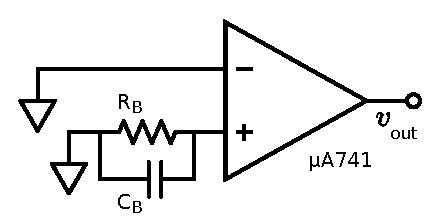
\includegraphics[width=0.30\textwidth]{../E02/latex/direct_measure.pdf}
  \end{center}
  \caption{Schema del circuito non retro-azionato utilizzato per stimare la corrente di polarizzazione. La resistenza utilizzata è $R_B=10.36\pm0.01$\si{\mega\ohm}; la capacità $C_B=102 \pm 1$ \si{\nano\farad}.}
  \label{circuito:rel2_correnti_senzaretroazione}
\end{wrapfigure}

Durante la procedura abbiamo però notato che, a causa di rumori ambientali, il valore di tensione sul multimetro fluttuava sulla prima cifra, rendendo nostra misurazione ovviamente non quantitativa (al massimo poteva stimarci l'ordine di grandezza della corrente). Per ovviare, abbiamo inserito in parallelo alla resistenza un condensatore che caricandosi si portava alla stessa ddp dei capi della resistenza. In questo modo abbiamo potuto ottenere un valore meno fluttuante, che si attestava a $V=(-80 \pm 2)$ \si{\milli\volt}, cioè $I_{b^+}=(7.7 \pm 0.2)$ \si{\nano\ampere}.

Con questo metodo semplice abbiamo potuto ottenere una prima stima del valore della corrente. Di contro bisogno considerare che il rumore non permette di avere una stima qualitativa ed inoltre la resistenza, scaldandosi, modifica il suo valore e potrebbe portare ad un errore sulla misura. Successivamente progetteremo dunque un circuito che, sfruttando l'amplificazione data dall'amplificatore operazionale, minimizzerà questi errori.

Analizziamo ora una possibile causa della  fluttuazione della misura.

\subsubsection*{Rumore termico}

Abbiamo considerato che la fluttuazione della misura sia dovuta ad un possibile effetto del rumore termico sulla nostra resistenza da \SI{10}{\mega\ohm}. Considerando la larghezza di banda del multimetro $\Delta f = \SI{1}{\hertz}$ e siano $k_B = \SI{1.38e-23}{\joule\per\kelvin}$ la costante di Boltzmann, $T$ la temperatura assoluta e $R$ il valore della resistenza presa in considerazione

\begin{equation}
	V_{eff}^2 = 4 k_B T R \Delta f
\end{equation}

da cui, ovviamente, si ottiene che il possibile rumore termico è 5 ordini di grandezza inferiore della tensione misurata

\begin{equation}
	V_{eff} = \sqrt{4 k_B T R \Delta f} \simeq 4 \times 10^{-7} \si{\volt}
\end{equation}

ed è pertanto ininfluente. Dunque il rumore presente è sicuramente imputabile ad altre cause ambientali.

\subsubsection{Configurazione con retroazione negativa}

\begin{wrapfigure}[15]{l}{0.55\textwidth}
  \begin{center}
    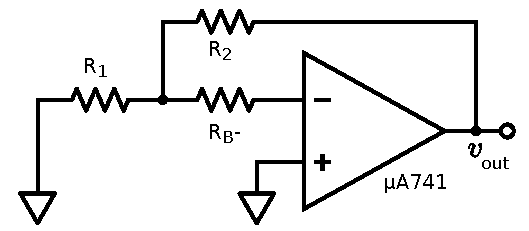
\includegraphics[width=0.35\textwidth]{../E02/latex/inv_current.pdf}
  \end{center}
  \caption{Schema del circuito retro-azionato utilizzato per stimare la corrente di polarizzazione $I_{b^-}$. Le resistenze utilizzate sono $R_1=(98.9\pm0.1)$ \si{\ohm}, $R_2=(99.4\pm0.1)$ \si{\kilo\ohm} e $R_B=(99.4\pm0.1)$ \si{\kilo\ohm}.}
  \label{circuito:rel2_correnti_retroazione_inv}
\end{wrapfigure}

Sfruttando un modello simile a quello utilizzato per trovare la tensione di offset, abbiamo montato i circuiti come in figura. Data la tensione in uscita, grazie alle proprietà di amplificazione dei segnali in ingresso dell'OPAMP, possiamo ottenere una misura indiretta della corrente di polarizzazione.

\subsubsection*{Misura di $I_{b^-}$}

Risolviamo il circuito per trovare la corrente di polarizzazione $I_{b^-}$ in funzione della tensione di uscita. Considerando $V_{-}$ la tensione al capo di $R_B$ collegato all'OPAMP e $V^*$ quello opposto, vale in quel punto la legge di Kirchhoff sui nodi

$$\frac{V^* - V_{in}}{R_1} + \frac{V^*-V_{out}}{R_2} + \frac{V^*-V_{-}}{R_B}=0$$

Dato che l'amplificatore operazionale è considerato già stabilizzato per quanto riguarda la tensione di offset, possiamo considerare la tensione all'ingresso invertente uguale all'ingresso non invertente. Vale dunque che $V_{in}=V_{-}=0$ e si trova (considerando $I_{b^-} R_B = V^*$):

$$I_{b^-}=\frac{V_{out}}{R_2 R_B}\frac{1}{\frac{1}{R_1}+\frac{1}{R_2}+\frac{1}{R_B}}$$

Le resistenze sono state dimensionate tenendo invece conto dell'ordine di grandezza della corrente da misurare e considerando il risultato sopra ottenuto: volevamo che $V_{out}$ fosse almeno $10^7\approx10^8$ volte più grande della corrente, per poter utilizzare il multimetro, che ha scale di misura limitate. I valori sono in Figura \ref{circuito:rel2_correnti_retroazione_inv}.

La misura di tensione di uscita è di $(3.89\pm0.02)$ \si{\volt} ed il valore ottenuto è dunque $I_{b^-} = (38 \pm 5)$ \si{\nano\ampere}.

\subsubsection*{Misura di $I_{b^+}$}

\begin{wrapfigure}[16]{r}{0.55\textwidth}
  \begin{center}
    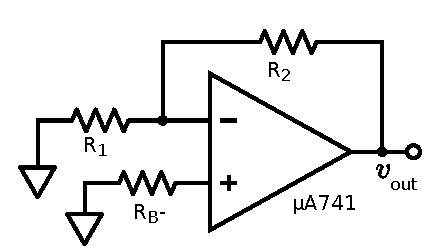
\includegraphics[width=0.25\textwidth]{../E02/latex/ninv_current.pdf}
  \end{center}
  \caption{Schema del circuito retro-azionato utilizzato per stimare la corrente di polarizzazione $I_{b^+}$. Le resistenze utilizzate sono le medesime del circuito precedente in Figura \ref{circuito:rel2_correnti_retroazione_inv}.}
  \label{circuito:rel2_correnti_retroazione_noninv}
\end{wrapfigure}

Similmente a quanto visto per la configurazione prima, troviamo che, data la legge di Kirchhoff (con $V^*$ la tensione all'ingresso non invertente, che per quanto detto sopra è uguale a quella all'ingresso invertente)

$$\frac{V^* - V_{in}}{R_1} + \frac{V^*-V_{out}}{R_2}=0$$

e considerando $V^*=I_{b^+} R_B$, otteniamo

\begin{equation}
I_{b^+}=\frac{V_{out}}{R_2 R_B}\frac{1}{\frac{1}{R_1}+\frac{1}{R_2}}
\label{eq2:corrente_noninv}
\end{equation}

Anche in questo caso le resistenze sono state dimensionate come sopra e i valori sono in Figura \ref{circuito:rel2_correnti_retroazione_noninv}. La misura di tensione di uscita è di $-(3.72 \pm 0.02)$   \si{\volt} ed il valore ottenuto è dunque $I_{b^+} = - (37.2 \pm 0.2)$ \si{\nano\ampere} \footnote{La negatività della corrente va intesa rispetto all'ingresso non invertente, ed è quindi uscente rispetto a tale ingresso. Al contrario, nel paragrafo precedente, la corrente è intesa entrante nel punto di $V^*$, e quindi è entrante rispetto all'ingresso invertente.}.

\subsubsection*{Calcolo di $I_{b^+}$ data $I_{b^-}$}

Consideriamo ora un altro modo per trovare la corrente di polarizzazione $I_{b^+}$ supponendo di aver già effettuato la misura di $I_{b^-}$ nel primo circuito (Figura \ref{circuito:rel2_correnti_retroazione_inv}). Successivamente controlleremo che il valore 'sperimentale' calcolato con (\ref{eq2:corrente_noninv}) è compatibile con quello calcolato in questo paragrafo.

Analizziamo dunque il secondo circuito (Figura \ref{circuito:rel2_correnti_retroazione_noninv}) per cercare di trovare la dipendenza di $I_{b^+}$ da $I_{b^-}$. Vale, dalla teoria, l'equazione (\ref{eq2:Vout_currents}), da cui è possibile ricavare

$$I_{b^+} = \frac{R_1}{R_B(R_1+R_2)}(I_{b^-} R_2-V_{out})$$

ed inserendo i valori otteniamo $I_{b^+} = - (37.2 \pm 0.2)$ \si{\nano\ampere}, compatibile con il risultato precedente.

\subsection{Conclusioni}
In questa esperienza abbiamo potuto osservare come gli OPAMP, sebbene siano dei circuiti abbastanza precisi, abbiano delle imperfezioni, date dalla loro composizione circuitale (sono presenti dei transistor BJT al loro interno).
Le discrepanze tra il modello ideale e l'OPAMP reale sono date principalmente dallo sbilanciamento della risposta dello stesso ($V_{offset}$) e dalle correnti di polarizzazione (\textit{bias currents}).
Per nostra fortuna spesso gli OPAMP presentano dei connettori predisposti a minimizzare la tensione di offset con circuiti di compensazione: nel nostro caso un trigger collegato ai piedini di offset e all'alimentazione negativa.
Una volta bilanciato l'opamp, abbiamo misurato le correnti di polarizzazione e abbiamo potuto osservare che esse sono dell'ordine dei \si{\nano\ampere}, quindi trascurabili per gli utilizzi più comuni.